\chapter{Testiranje i vrednovanje rješenja}

Nakon implementacije aplikacije, potrebno je provesti testiranje u realnim uvjetima kako bi se validirala funkcionalnost te procijenile performanse i praktična upotreba. Cilj poglavlja je analizirati rezultate testiranja, s posebnim naglaskom na funkcionalnost prepoznavanja penjačkih smjerova, te identificirati ograničenja i područja za poboljšanje.

\section{Metodologija testiranja}

Testiranje je provedeno na penjalištu Kalnik, koje zbog svoje popularnosti i raznolikosti stijena predstavlja prikladnu lokaciju za ispitivanje sustava. Za detaljnu analizu odabrana su dva penjačka smjera s različitim vizualnim karakteristikama kako bi se ispitala robusnost algoritma. 

\begin{figure}[H]
    \centering
    \begin{subfigure}[b]{0.45\textwidth}
        \centering
        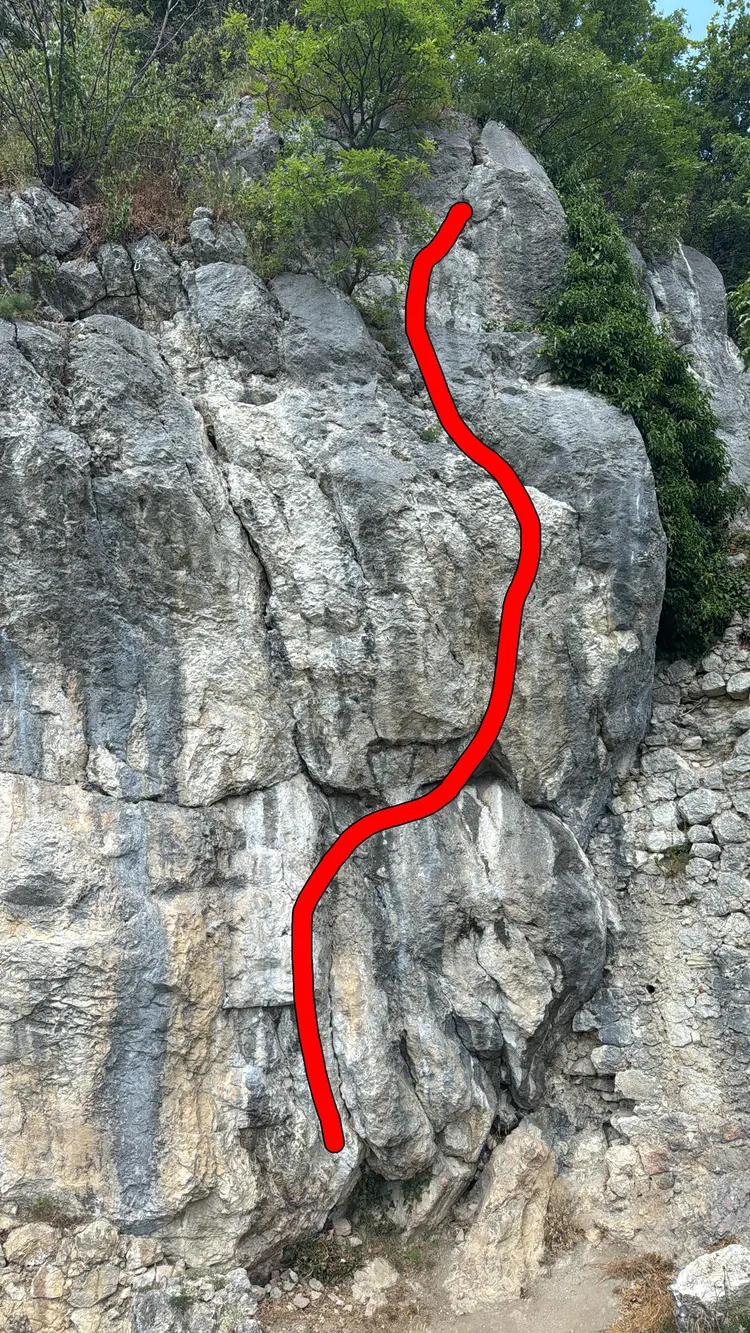
\includegraphics[width=\textwidth]{images/testiranje/apaches_ref_slika.png}
        \caption{Referentna slika smjera "Apaches"}
        \label{fig:apaches}
    \end{subfigure}
    \hfill
    \begin{subfigure}[b]{0.45\textwidth}
        \centering
        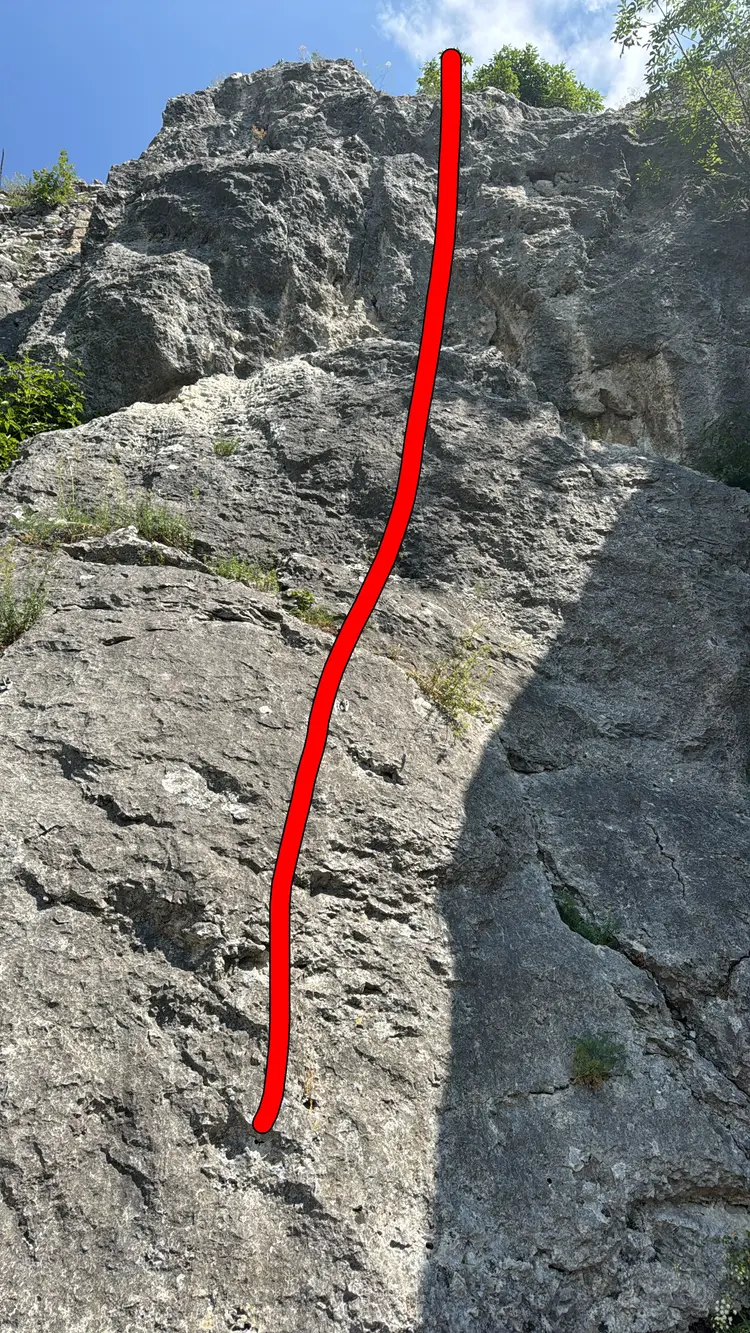
\includegraphics[width=\textwidth]{images/testiranje/steyr_ref.png}
        \caption{Referentna slika smjera "Steyr"}
        \label{fig:steyr}
    \end{subfigure}
    \caption{Referentne slike odabranih penjačkih smjerova na penjalištu Kalnik}
    \label{fig:referentne_slike}
\end{figure}

Prvi primjer penjačkog smjera je "Apaches" u sektoru Stari Grad B (Slika~\ref{fig:apaches}). Smjer je lako prepoznatljiv zbog mnogo distinktnih značajki poput rupa, pukotina i varijacija u boji. Drugi primjer je smjer "Steyr" u sektoru Stari Grad A (Slika~\ref{fig:steyr}). Za razliku od "Apaches", smjer se nalazi na relativno glatkoj i uniformnoj stijeni s manje izraženih značajki, što predstavlja izazov za algoritam.

Za oba smjera prethodno su, putem aplikacije, kreirane referentne slike s ucrtanim linijama. Testiranje je izvršeno na uređaju iPhone 15 Pro u automatskom načinu rada primarno na "High" razini prepoznavanja, no također su testirane i niže razine "Medium" i "Low".


\section{Rezultati i analiza funkcionalnosti}

Sustav je u praksi potvrdio svoju funkcionalnost. Na smjeru "Apaches", koji je bogat značajkama, aplikacija brzo i stabilno prepoznaje stijenu te precizno projicira virtualnu liniju smjera preko video prikaza čak i iz različitih kutova (Slika~\ref{fig:apaches_test_double}) i korištenjem nižih razina prepoznavanja.

\begin{figure}[H]
    \centering
    \begin{subfigure}[b]{0.45\textwidth}
        \centering
        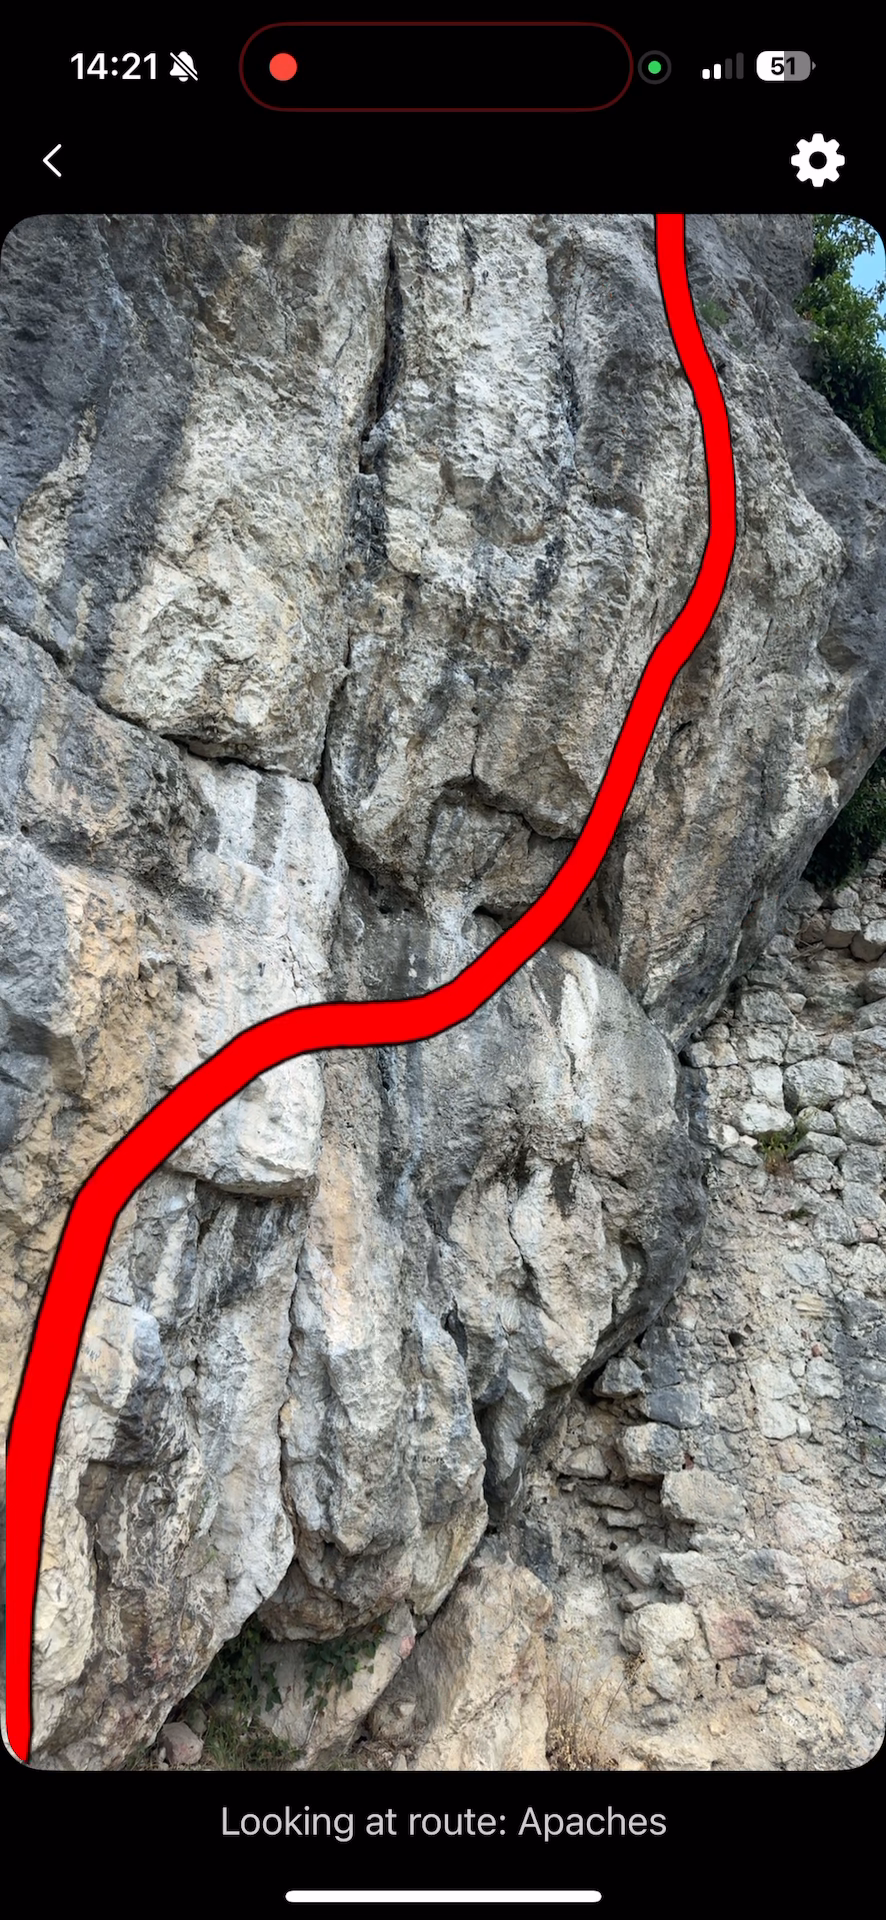
\includegraphics[width=\textwidth]{images/testiranje/apaches_test_left_side.png}
        \caption{Testiranje smjera "Apaches" s lijeve strane}
        \label{fig:apaches_test_left_side}
    \end{subfigure}
    \hfill
    \begin{subfigure}[b]{0.45\textwidth}
        \centering
        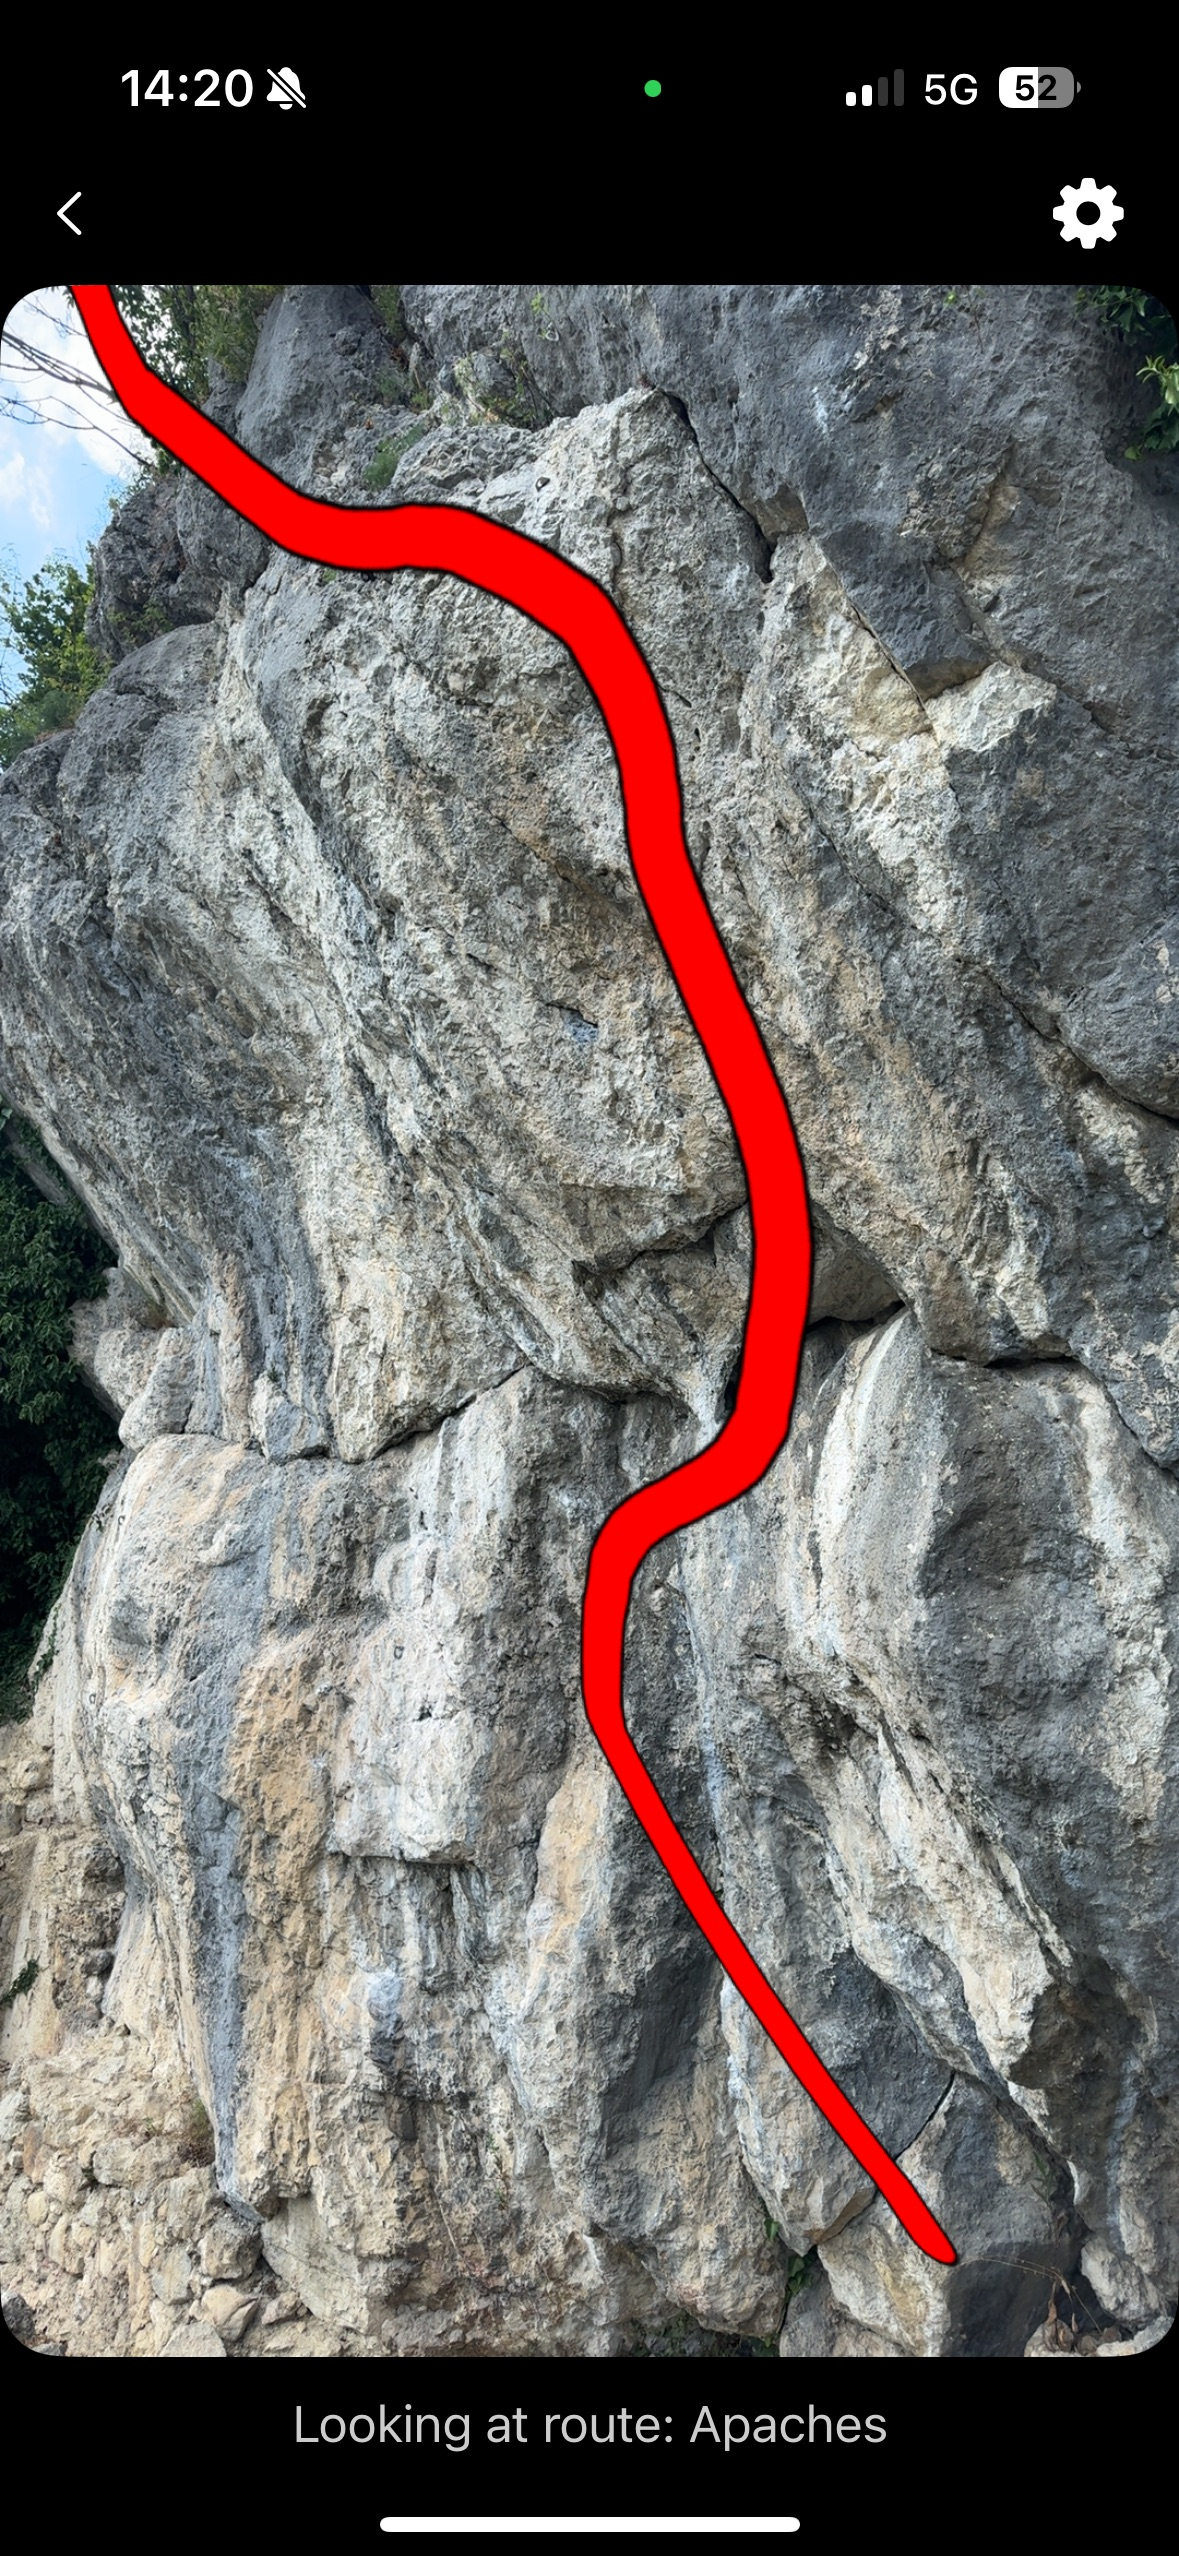
\includegraphics[width=\textwidth]{images/testiranje/apaches_test_right_side.jpeg}
        \caption{Testiranje smjera "Apaches" s desne strane}
        \label{fig:apaches_test_right_side}
    \end{subfigure}
    \caption{Testiranje smjera "Apaches" iz dva različita kuta}
    \label{fig:apaches_test_double}
\end{figure}

Testiranje je na zahtjevnijem smjeru "Steyr" također rezultiralo u uspješnom detekcijom (Slika~\ref{fig:steyr_test_double}), no učeno je da je za stabilno prepoznavanje bilo potrebno pažljivije i strpljivije usmjeravanje kamere prema stijeni kako bi linija smjera bila preciznije pozicionirana. 

\begin{figure}[H]
    \centering
    \begin{subfigure}[b]{0.45\textwidth}
        \centering
        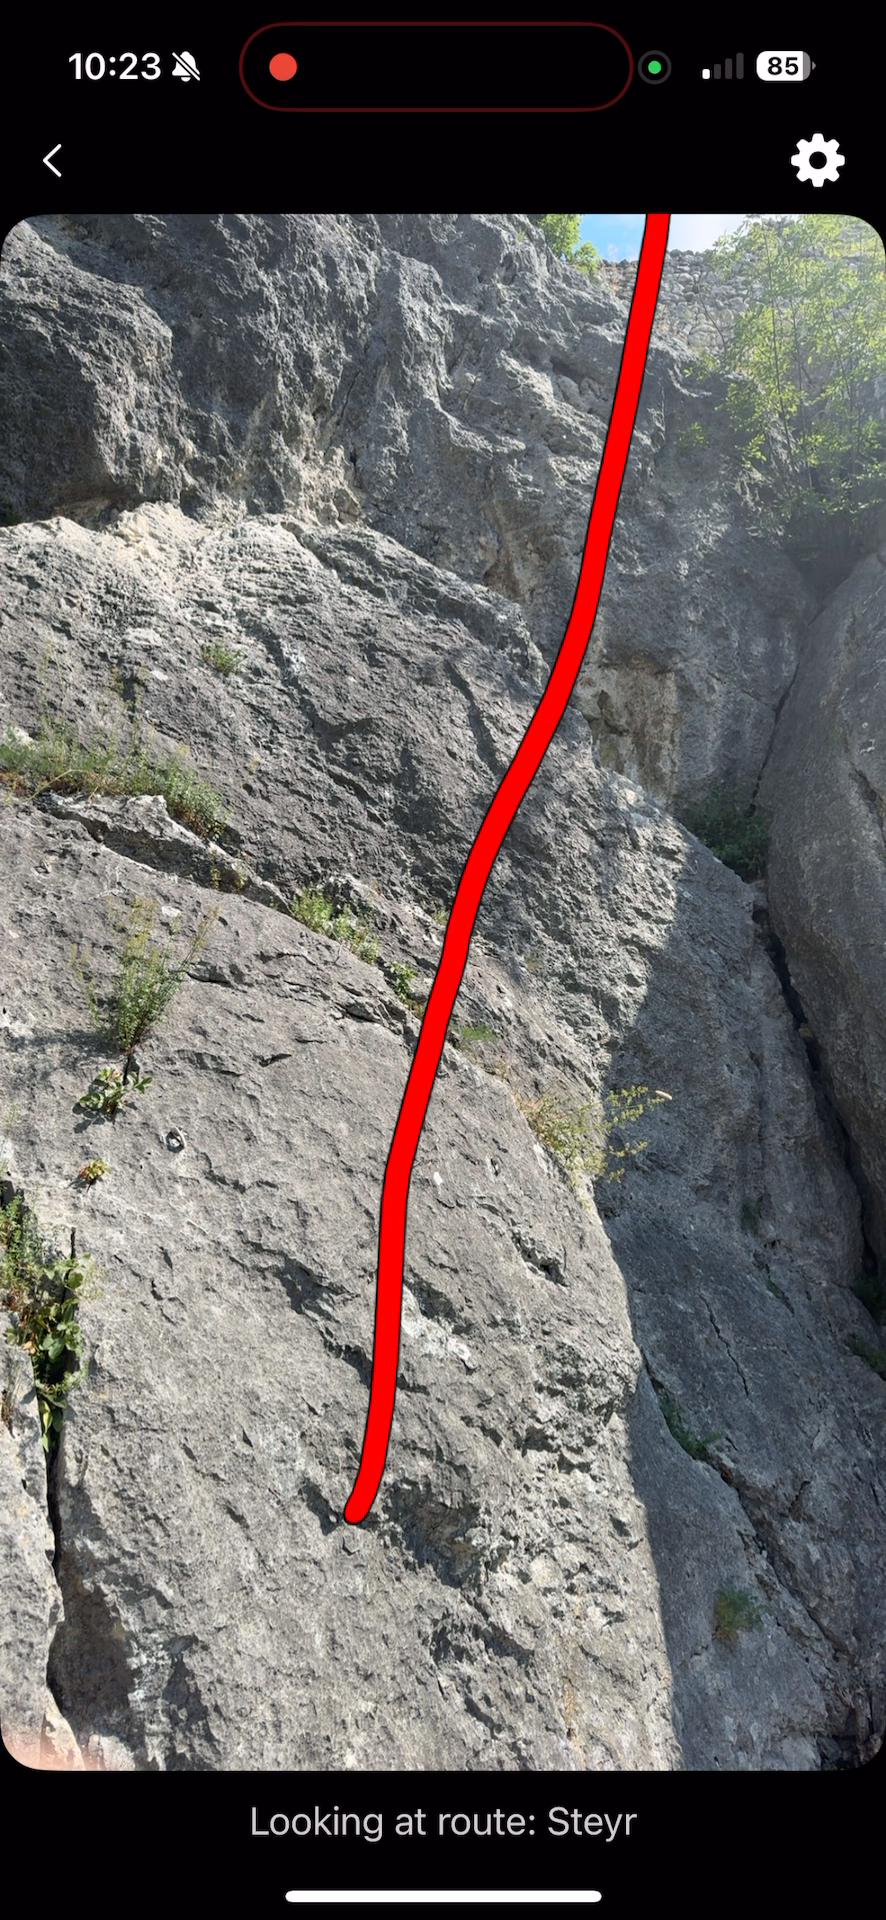
\includegraphics[width=\textwidth]{images/testiranje/steyr_test_left_side.png}
        \caption{Testiranje smjera "Steyr" s lijeve strane}
        \label{fig:steyr_test_left_side}
    \end{subfigure}
    \hfill
    \begin{subfigure}[b]{0.45\textwidth}
        \centering
        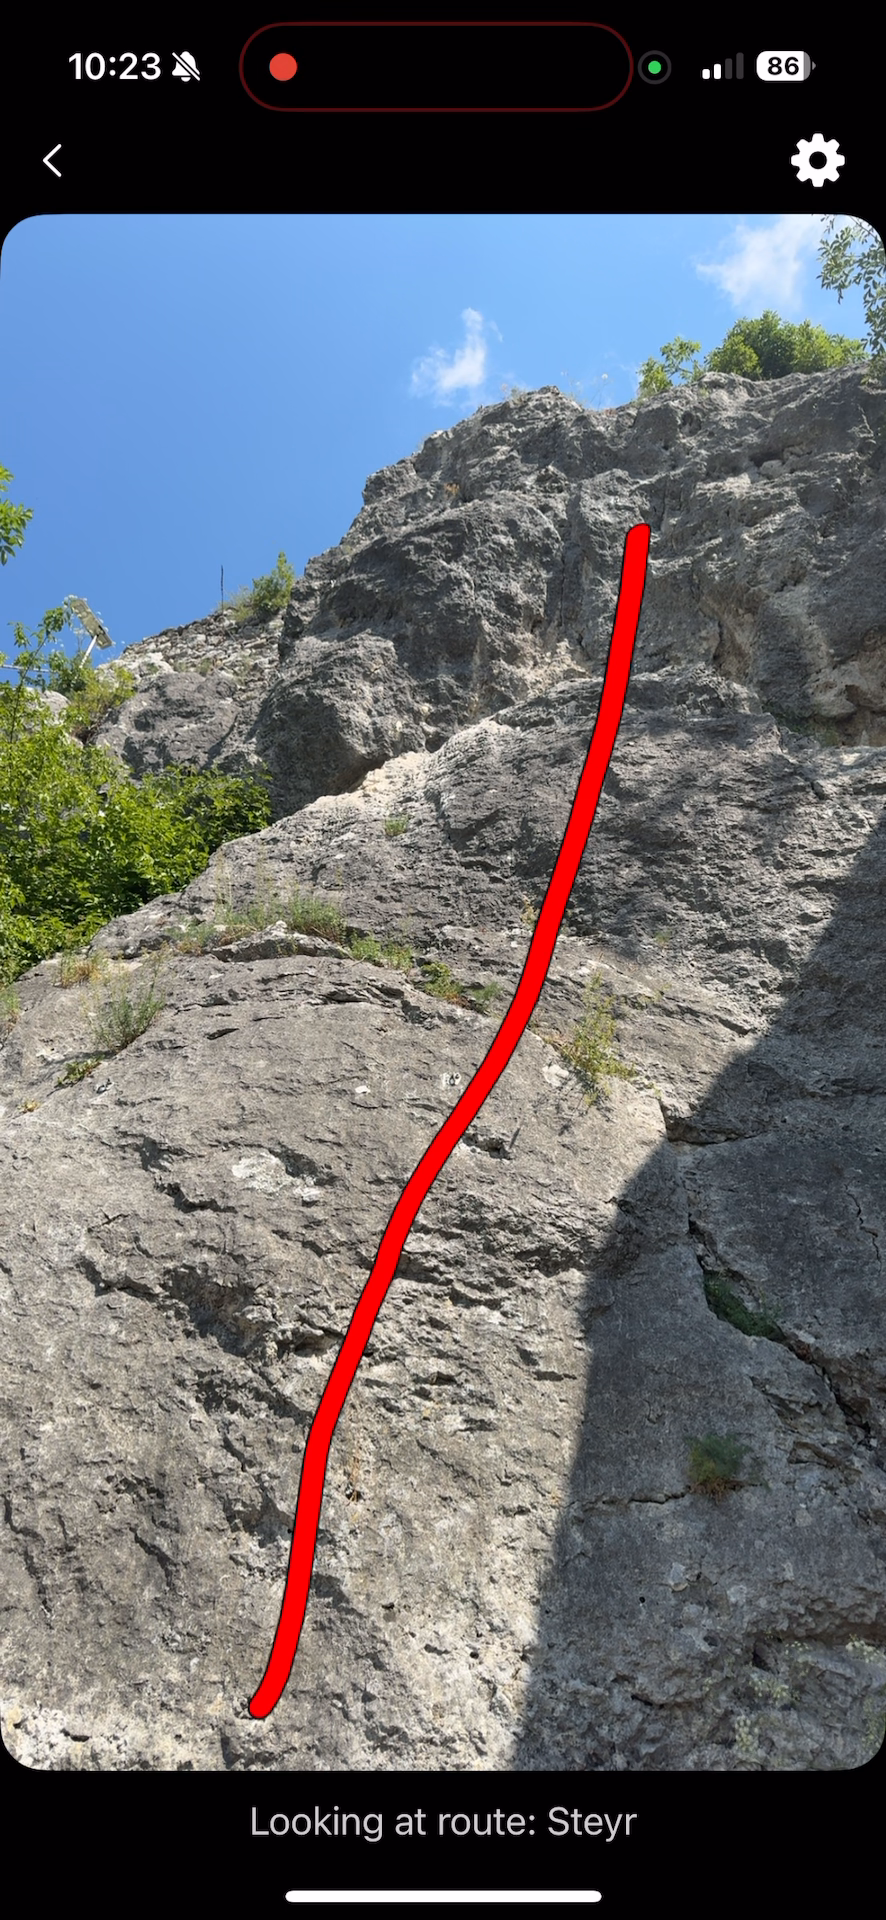
\includegraphics[width=\textwidth]{images/testiranje/steyr_test_right_side.png}
        \caption{Testiranje smjera "Steyr" s desne strane}
        \label{fig:steyr_test_right_side}
    \end{subfigure}
    \caption{Testiranje smjera "Steyr" iz dva različita kuta}
    \label{fig:steyr_test_double}
\end{figure}

\section{Analiza performansi i uočenih problema}

Unatoč uspješnoj funkcionalnoj validaciji, testiranje je otkrilo nekoliko problema vezanih uz performanse i korisničko iskustvo.

\begin{figure}[H]
    \centering
    \begin{subfigure}[b]{0.45\textwidth}
        \centering
        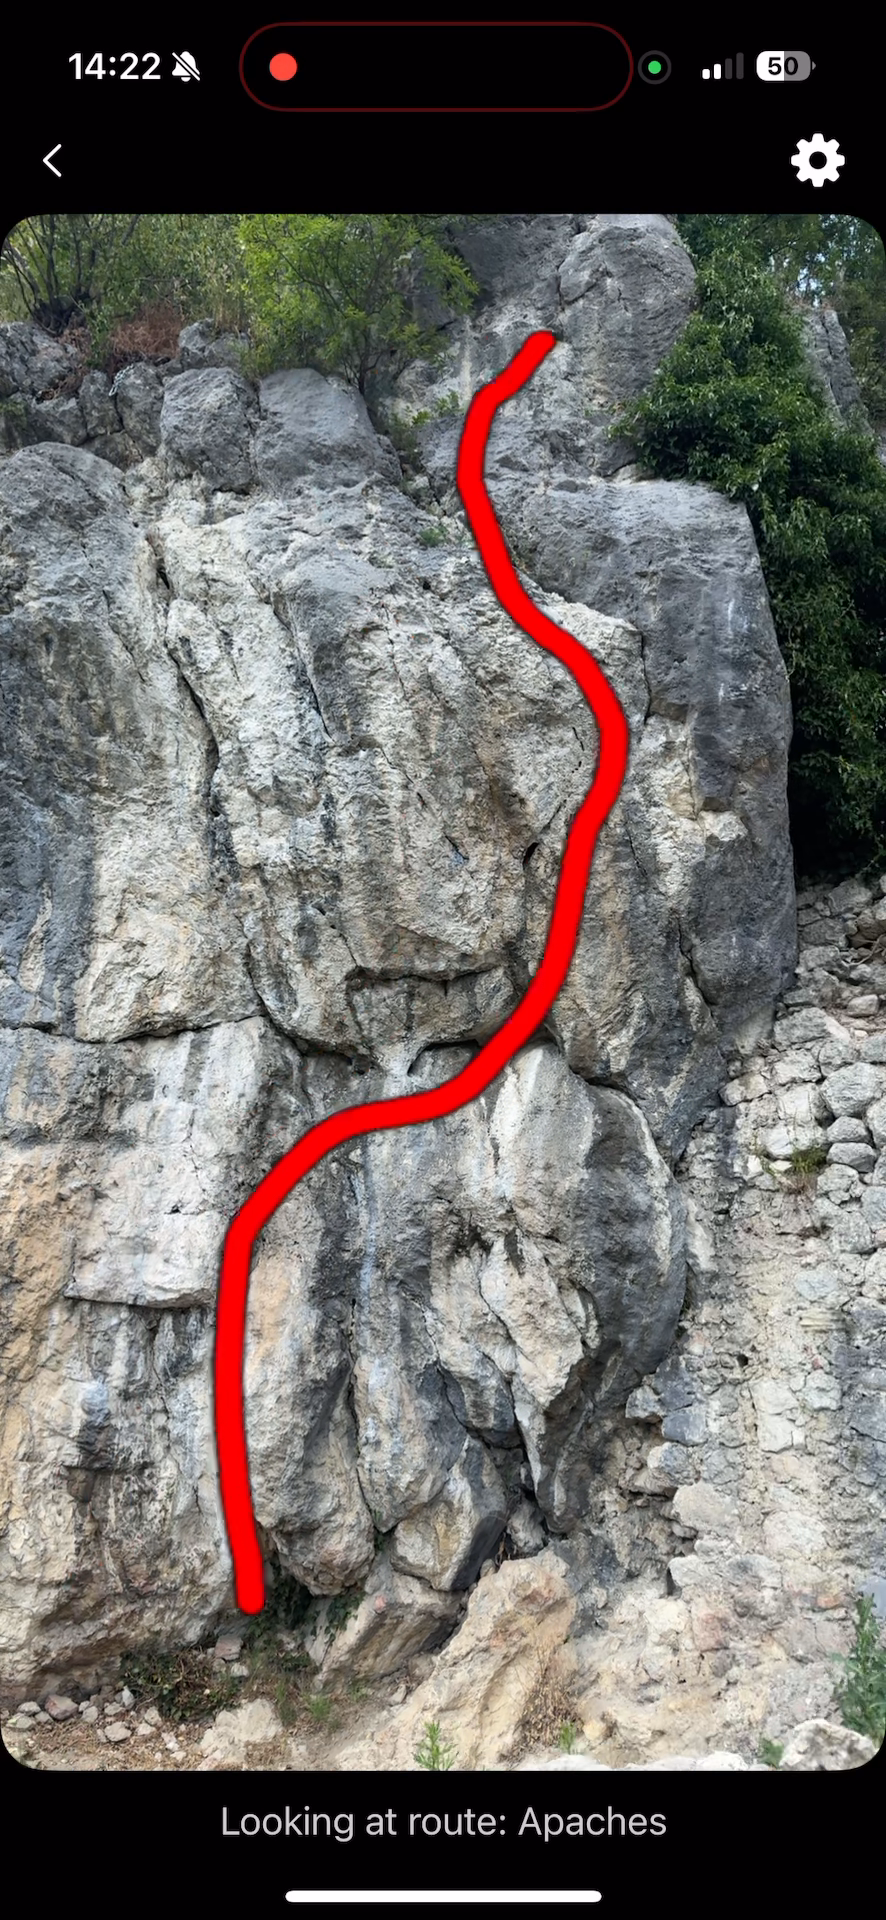
\includegraphics[width=\textwidth]{images/testiranje/apaches_latency_before.png}
        \caption{Prije pomicanja kamere}
        \label{fig:apaches_latency_before}
    \end{subfigure}
    \hfill
    \begin{subfigure}[b]{0.45\textwidth}
        \centering
        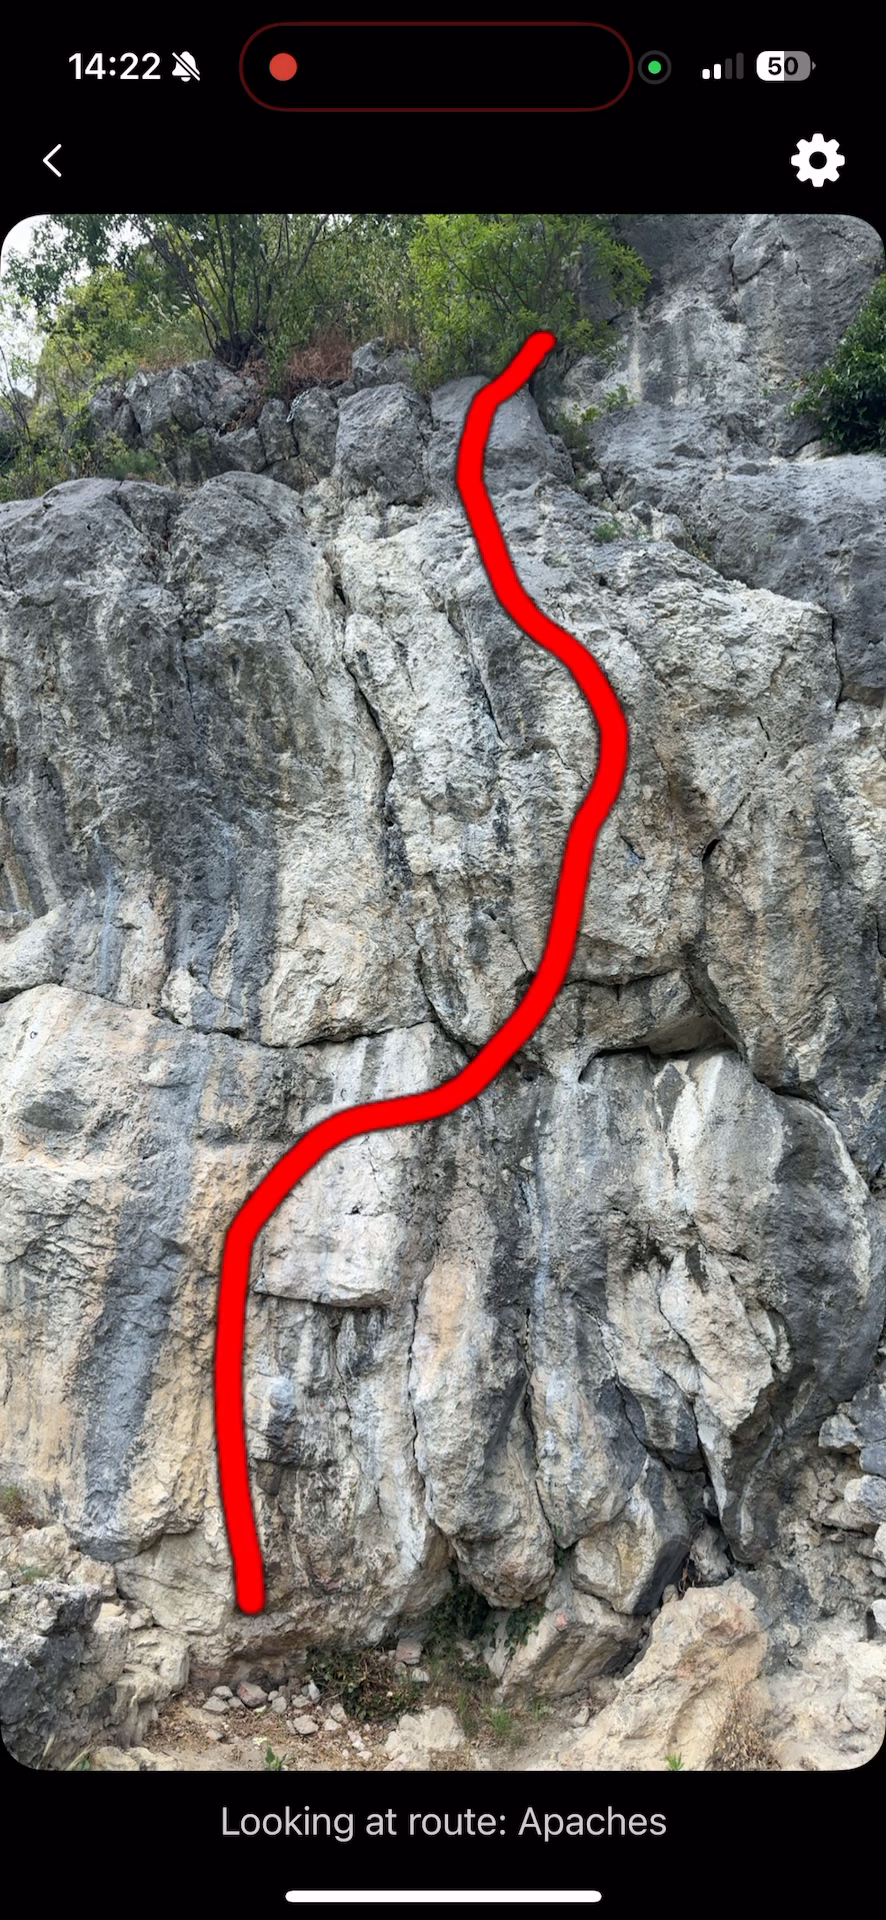
\includegraphics[width=\textwidth]{images/testiranje/apaches_latency_after.png}
        \caption{Nakon pomicanja kamere}
        \label{fig:apaches_latency_after}
    \end{subfigure}
    \caption{Primjeri latencije kod detekcije smjera "Apaches"}
    \label{fig:apaches_latency_double}
\end{figure}

Prvi uočeni nedostatak je kašnjenje ili latencija između fizičkog pomicanja kamere i ažuriranje položaja virtualne linije na ekranu što prikazuje slika~\ref{fig:apaches_latency_double}. Ovo kašnjenje je posljedica računske zahtjevnosti SIFT algoritma i cjelokupnog procesa obrade koji se izvršava na mobilnom uređaju. Problem je izražen pri korištenju "High" postavke jačine prepoznavanja, gdje je kašnjenje bilo vidljivo i ometajuće, dok je na "Low" postavci bilo manje primjetno, ali uz smanjenu preciznost. 
Važan uvid dobiven testiranjem, a isto vezan uz problem latencije, odnosi se na odluku o upravljanju kadrovima dobivenim s kamere. Inicijalna implementacija koristila je \textit{AsyncStream} s politikom \textit{bufferingOldest(1)}, s idejom da nije bitno je li se koristi \textit{bufferingOldest(1)} ili \textit{bufferingNewest(1)} jer se u idealnim uvjetima pokazalo da brzina obrade nije toliko mala da ima značaja. Međutim, u realnim uvjetima, posebice na "High" postavci, obrada jednog kadra traje znatno duže od intervala između dva kadra. Korištenje \textit{bufferingOldest} politike u takvom scenariju dovodi do lošijih detekcija jer se koristi stariji kadar, a ne najnoviji. Time bi aplikacija prikazivala virtualnu liniju izračunatu na temelju kadra koji ne predstavlja najnoviji kadar.

\begin{figure}[H]
    \centering
    \begin{subfigure}[b]{0.45\textwidth}
        \centering
        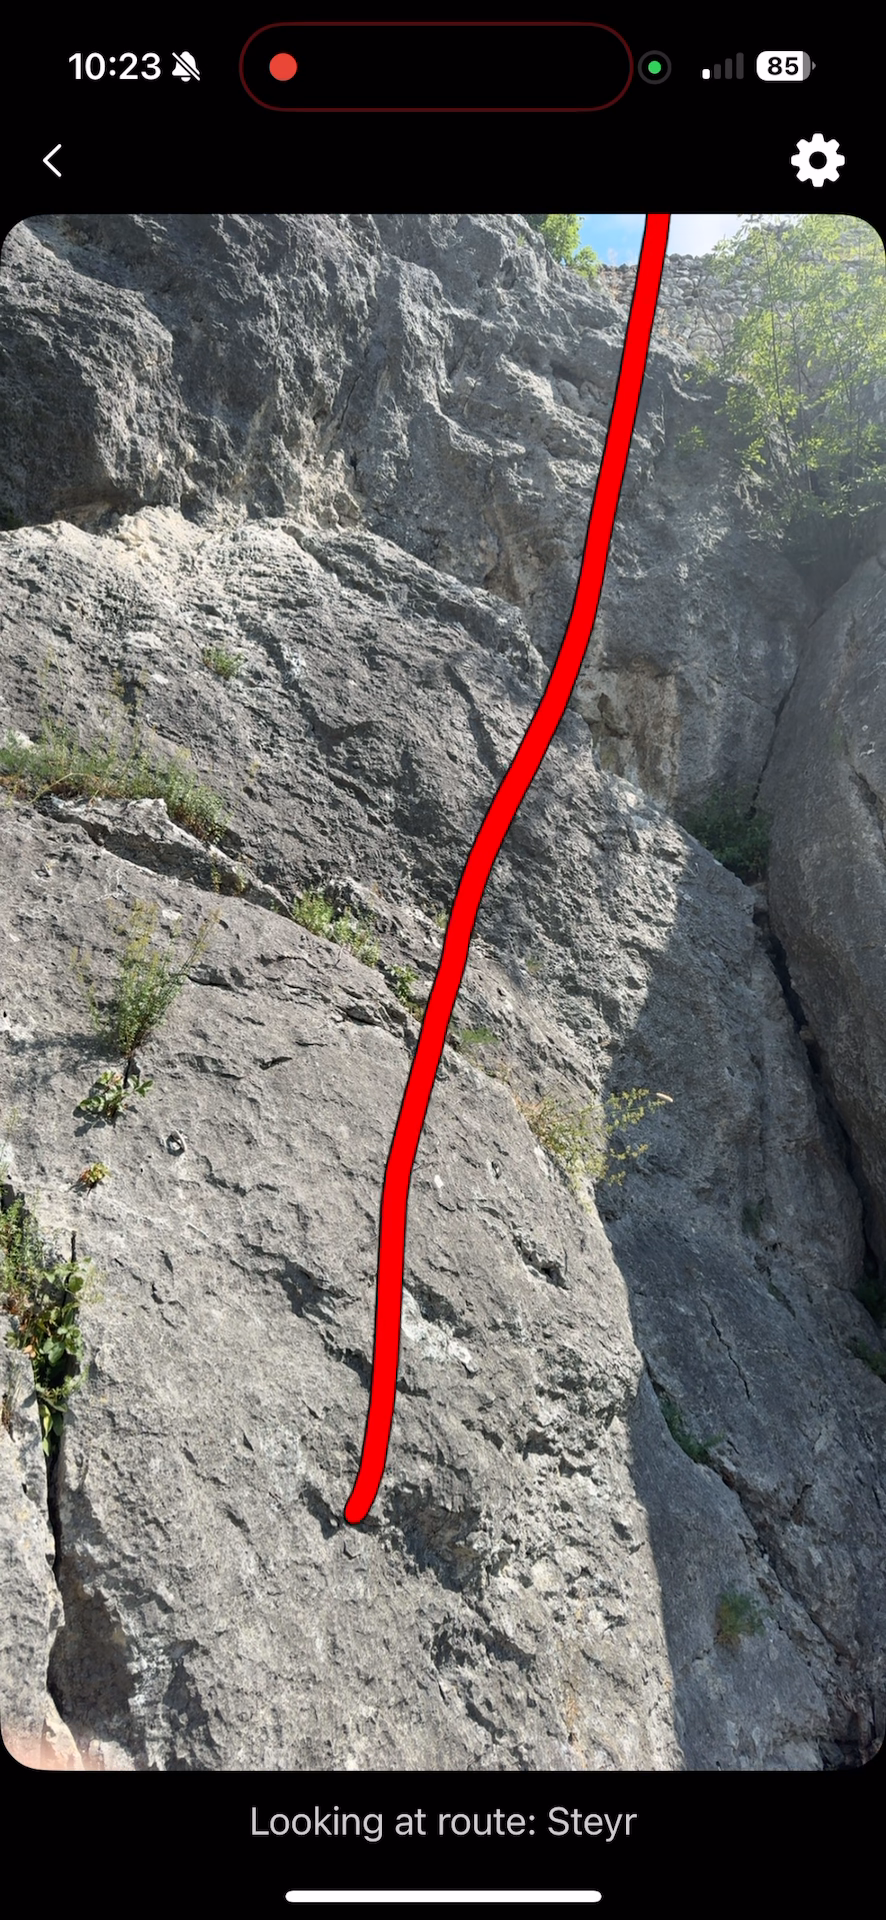
\includegraphics[width=\textwidth]{images/testiranje/steyr_bad_detection_before_moving.png}
        \caption{Prije pomicanja kamere}
        \label{fig:steyr_bad_detection_2a}
    \end{subfigure}
    \hfill
    \begin{subfigure}[b]{0.45\textwidth}
        \centering
        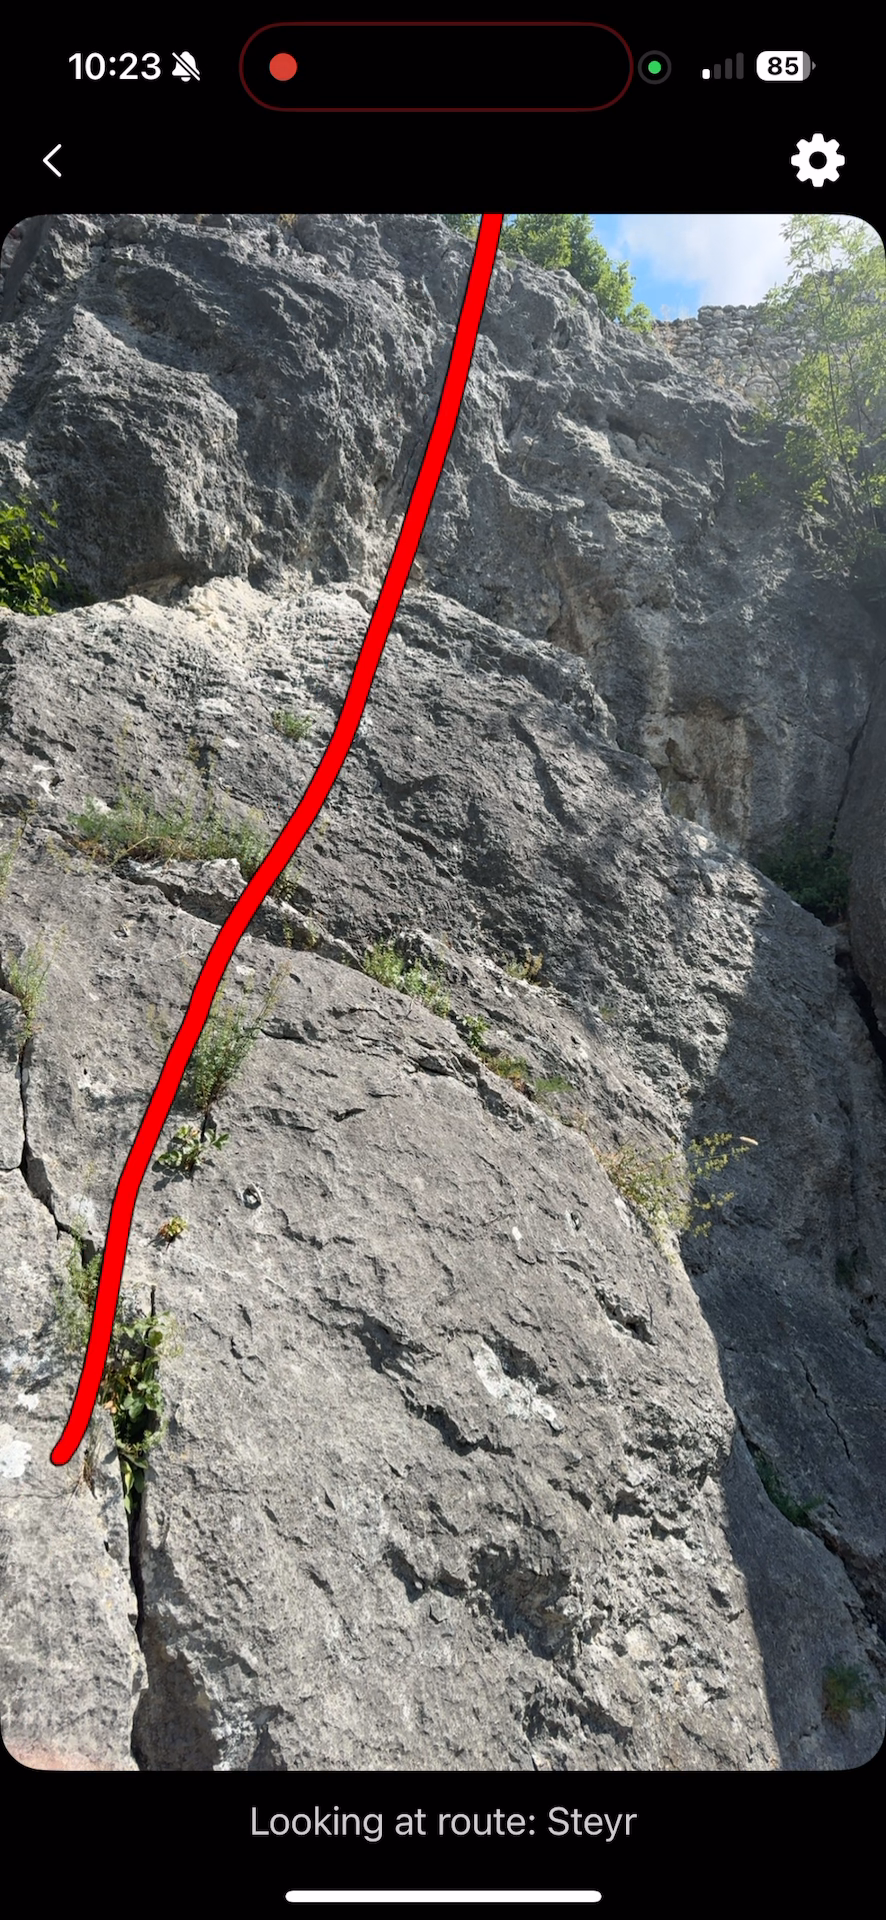
\includegraphics[width=\textwidth]{images/testiranje/steyr_bad_detection_after_moving.png}
        \caption{Nakon pomicanja kamere}
        \label{fig:steyr_bad_detection_2b}
    \end{subfigure}
    \caption{Primjeri posljedice korištenja \textit{bufferingOldest(1)} politike}
    \label{fig:steyr_bad_detection_double_2}
\end{figure}

Slika~\ref{fig:steyr_bad_detection_double_2} prikazuje primjere posljedice korištenja \textit{bufferingOldest(1)} politike. Na slici~\ref{fig:steyr_bad_detection_2a} prikazan je primjer prije pomicanja kamere, a na slici~\ref{fig:steyr_bad_detection_2b} nakon pomicanja kamere. Vidljivo je da se virtualna linija pojavila na pogrešnoj lokaciji prije nego što bi se stabilizirala na ispravnoj poziciji. Pogreška dolazi zbog sljedeće situacije. Kada je završila detekcija, proces detekcije uzima kadar iz spremnika i kreće obradu. Sljedeći kadar koji dolazi s kamere se sprema u spremnik i ne spremaju se novi kadrovi. Kada dolazi vrijeme za obradu novog kadra, uzima se taj stariji kadar. Korištenjem \textit{bufferingNewest(1)} politike, svaki novi kadar zamijenjuje kadar iz spremnika, što bi minimiziralo ovaj problem jer bi se obradio kadar koji je netom došao s kamere.



Drugi uočeni problem je nestabilnost detekcije. Tijekom korištenja, virtualna linija bi se kratkotrajno pojavila na pogrešnoj lokaciji prije nego što bi se stabilizirala na ispravnoj poziciji. Slika~\ref{fig:steyr_bad_detection_double_3} prikazuje primjer nestabilnosti detekcije smjera "Steyr".

\begin{figure}[H]
    \centering
    \begin{subfigure}[b]{0.45\textwidth}
        \centering
        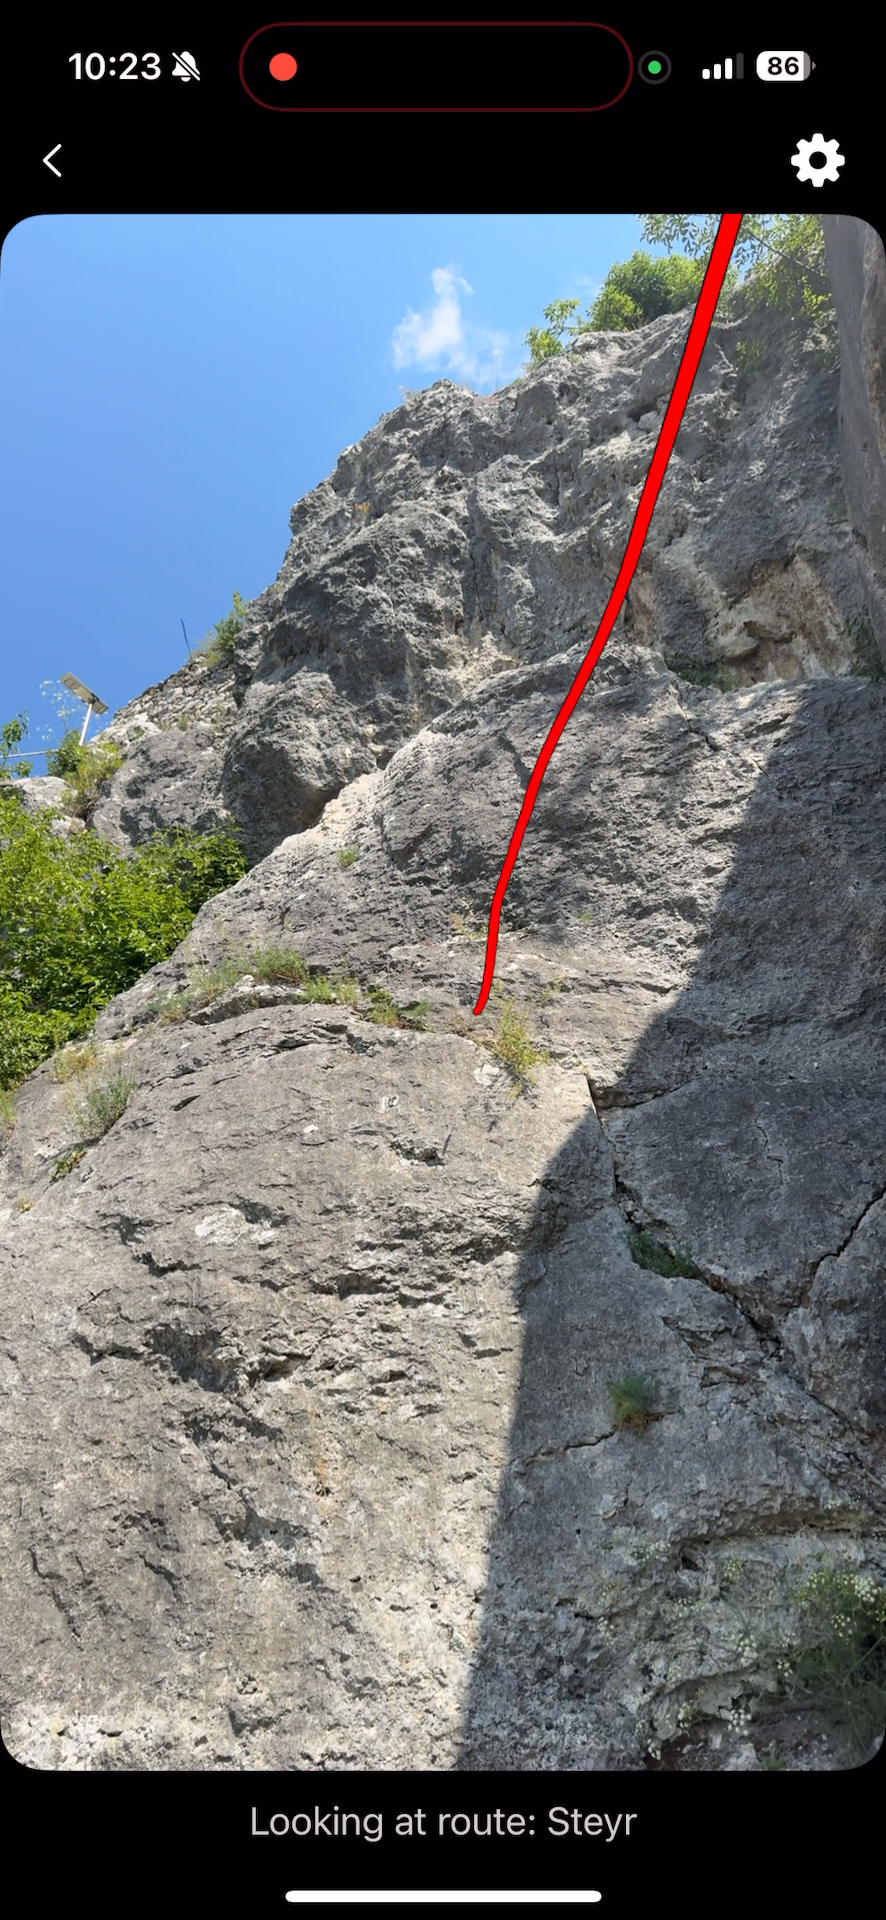
\includegraphics[width=\textwidth]{images/testiranje/steyr_bad_detection_before_homography_fix.png}
        \caption{Prije ispravka}
        \label{fig:steyr_bad_detection_before_fix}
    \end{subfigure}
    \hfill
    \begin{subfigure}[b]{0.45\textwidth}
        \centering
        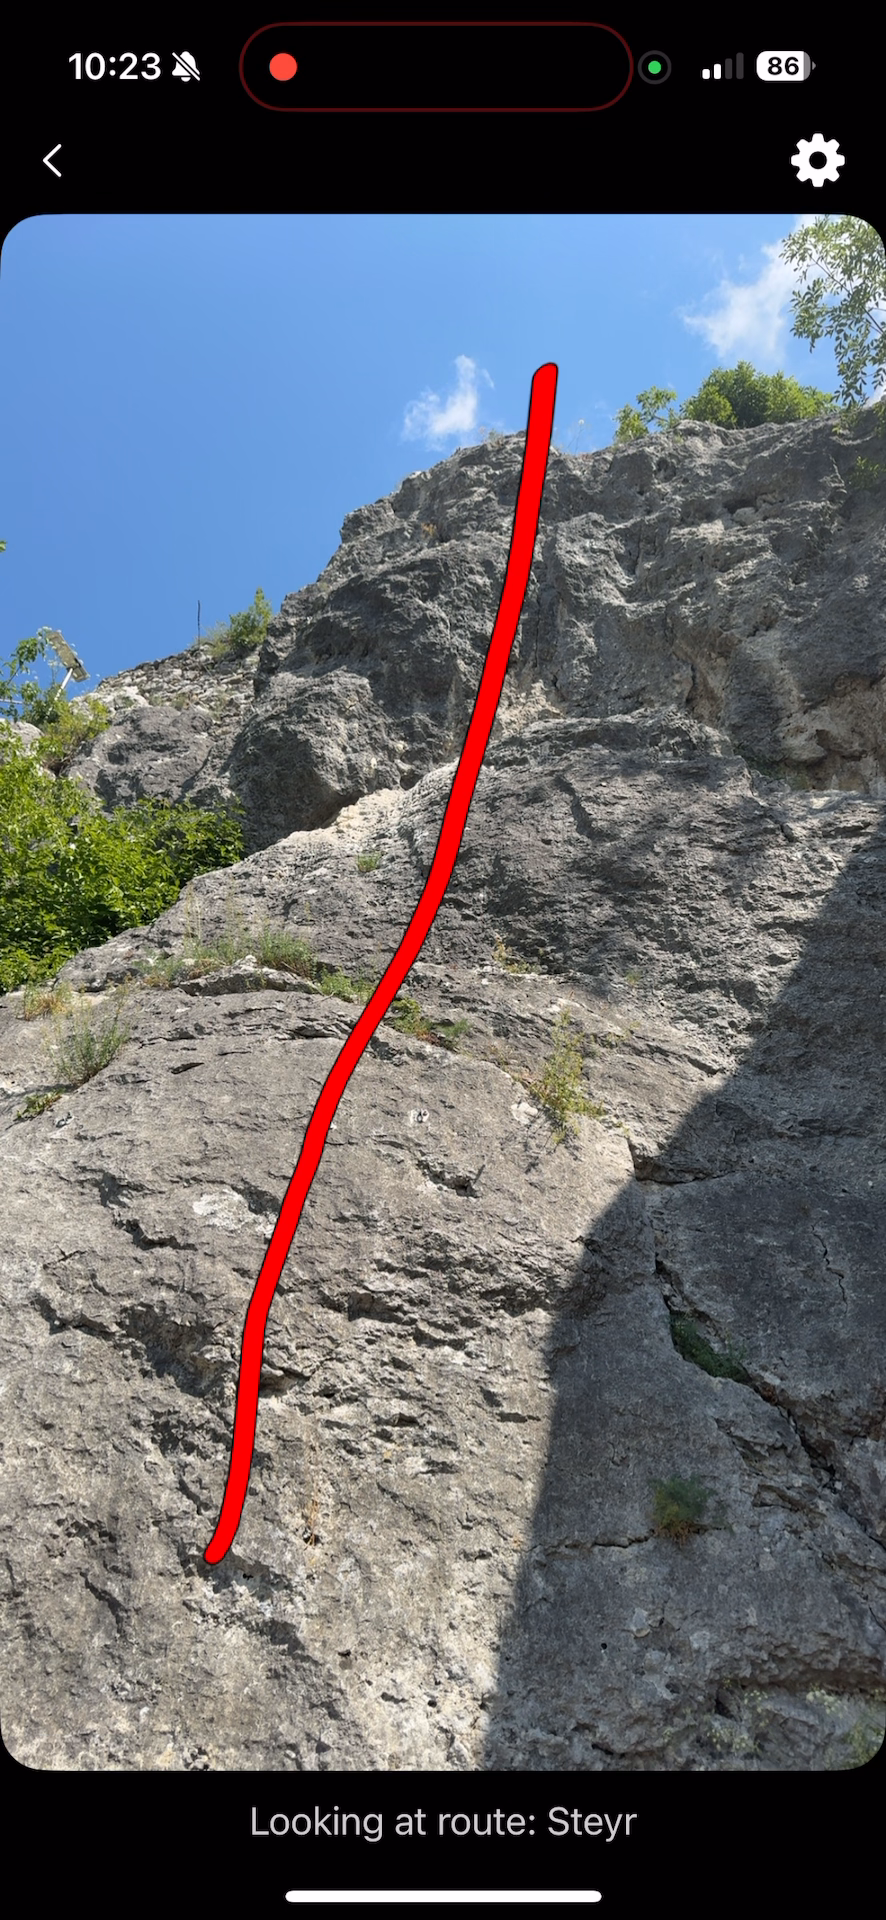
\includegraphics[width=\textwidth]{images/testiranje/steyr_bad_detection_after_homography_fix.png}
        \caption{Nakon ispravka}
        \label{fig:steyr_bad_detection_after_fix}
    \end{subfigure}
    \caption{Primjer nestabilnosti detekcije smjera "Steyr"}
    \label{fig:steyr_bad_detection_double_3}
\end{figure}


Ovaj fenomen nastaje u trenucima kada algoritam pronađe prividno dovoljan broj podudarnosti koje su zapravo pogrešne, ali ih RANSAC algoritam privremeno prihvati kao valjan model. Slično se događa kada korisnik zapravo ne gleda u smjer, već negdje drugdje i na trenutak se pojavi linija penjačkog smjera. Iako se sustav oporavi i pronalazi ispravnu homografiju, ova nestabilnost može smanjiti povjerenje korisnika u sustav. 

